\label{sec:relatedworks}
\subsection{Описание предметной области}
Входящие в состав клеток всех живых существ макромолекулы --- нуклеиновые кислоты и белки --- имеют очень разнообразные биологические функции и играют важные роли во множестве процессов, определяющих жизнедеятельность и эволюционное развитие организмов. Со структурной точки зрения их объединяет то, что они являются полимерами, т.е. состоят из некоторых элементарных единиц --- мономеров, --- соединенных в крупные молекулы по определенным законам.  Как ДНК и РНК, так и белки имеют несколько уровней организации, т.е. характеризуются линейной (первичной) структурой, которая представляет собой последовательность из мономеров, и пространственной (вторичной), основанной на молекулярных взаимодействиях между ними. 

В частности, молекула РНК состоит из цепи особых веществ --- нуклеотидов четырех типов, которые называются аденин, гуанин, цитозин и урацил (A, G, C, U) и могут образовывать между собой попарные водородные связи. Законы формирования нуклеотидных пар обусловлены поддержанием термодинамического равновесия вторичной структуры, и самыми стабильными и распространенными в природе являются канонические, Уотсон-Криковские, пары $A-U$, $C-G$, однако с разной степенью вероятности могут встречаться и любые другие комбинации. Способность нуклеотидов формировать связи приводит к склеиванию определенных участков цепи РНК между собой и образованию вторичной структуры, базовым элементом которой является так называемая шпилька, которая образуется в том случае, когда две последовательности одной и той же цепи соединяются друг с другом, перегибаясь одна к другой и образуя на конце неспаренный участок --- петлю. Пример элементарной шпильки высоты четыре, образованной только каноническими парами, показан на рис.~\ref{rna_a}, и вторичная структура РНК в целом может быть представлена как рекурсивная композиция шпилек варьирующегося размера~\cite{quadrini2019loop}. В различных работах по биоинформатике можно встретить разделение элементов вторичной структуры по внешнему виду на несколько типов (hairpin, internal loop, bulge, helix, multi-loop и др.), однако формально все эти элементы могут быть определены через вложенные шпильки (рис.~\ref{rna_b}). Особый интерес представляют псевдоузлы (pseudoknots), состоящие из двух шпилек, где половина стебля одной из них располагается между двумя половинами стебля другой, и имеющее большое функциональное значение для живых организмов. 

\begin{figure}[h]
\centering
\begin{subfigure}{.5\textwidth}
  \centering
  \fbox{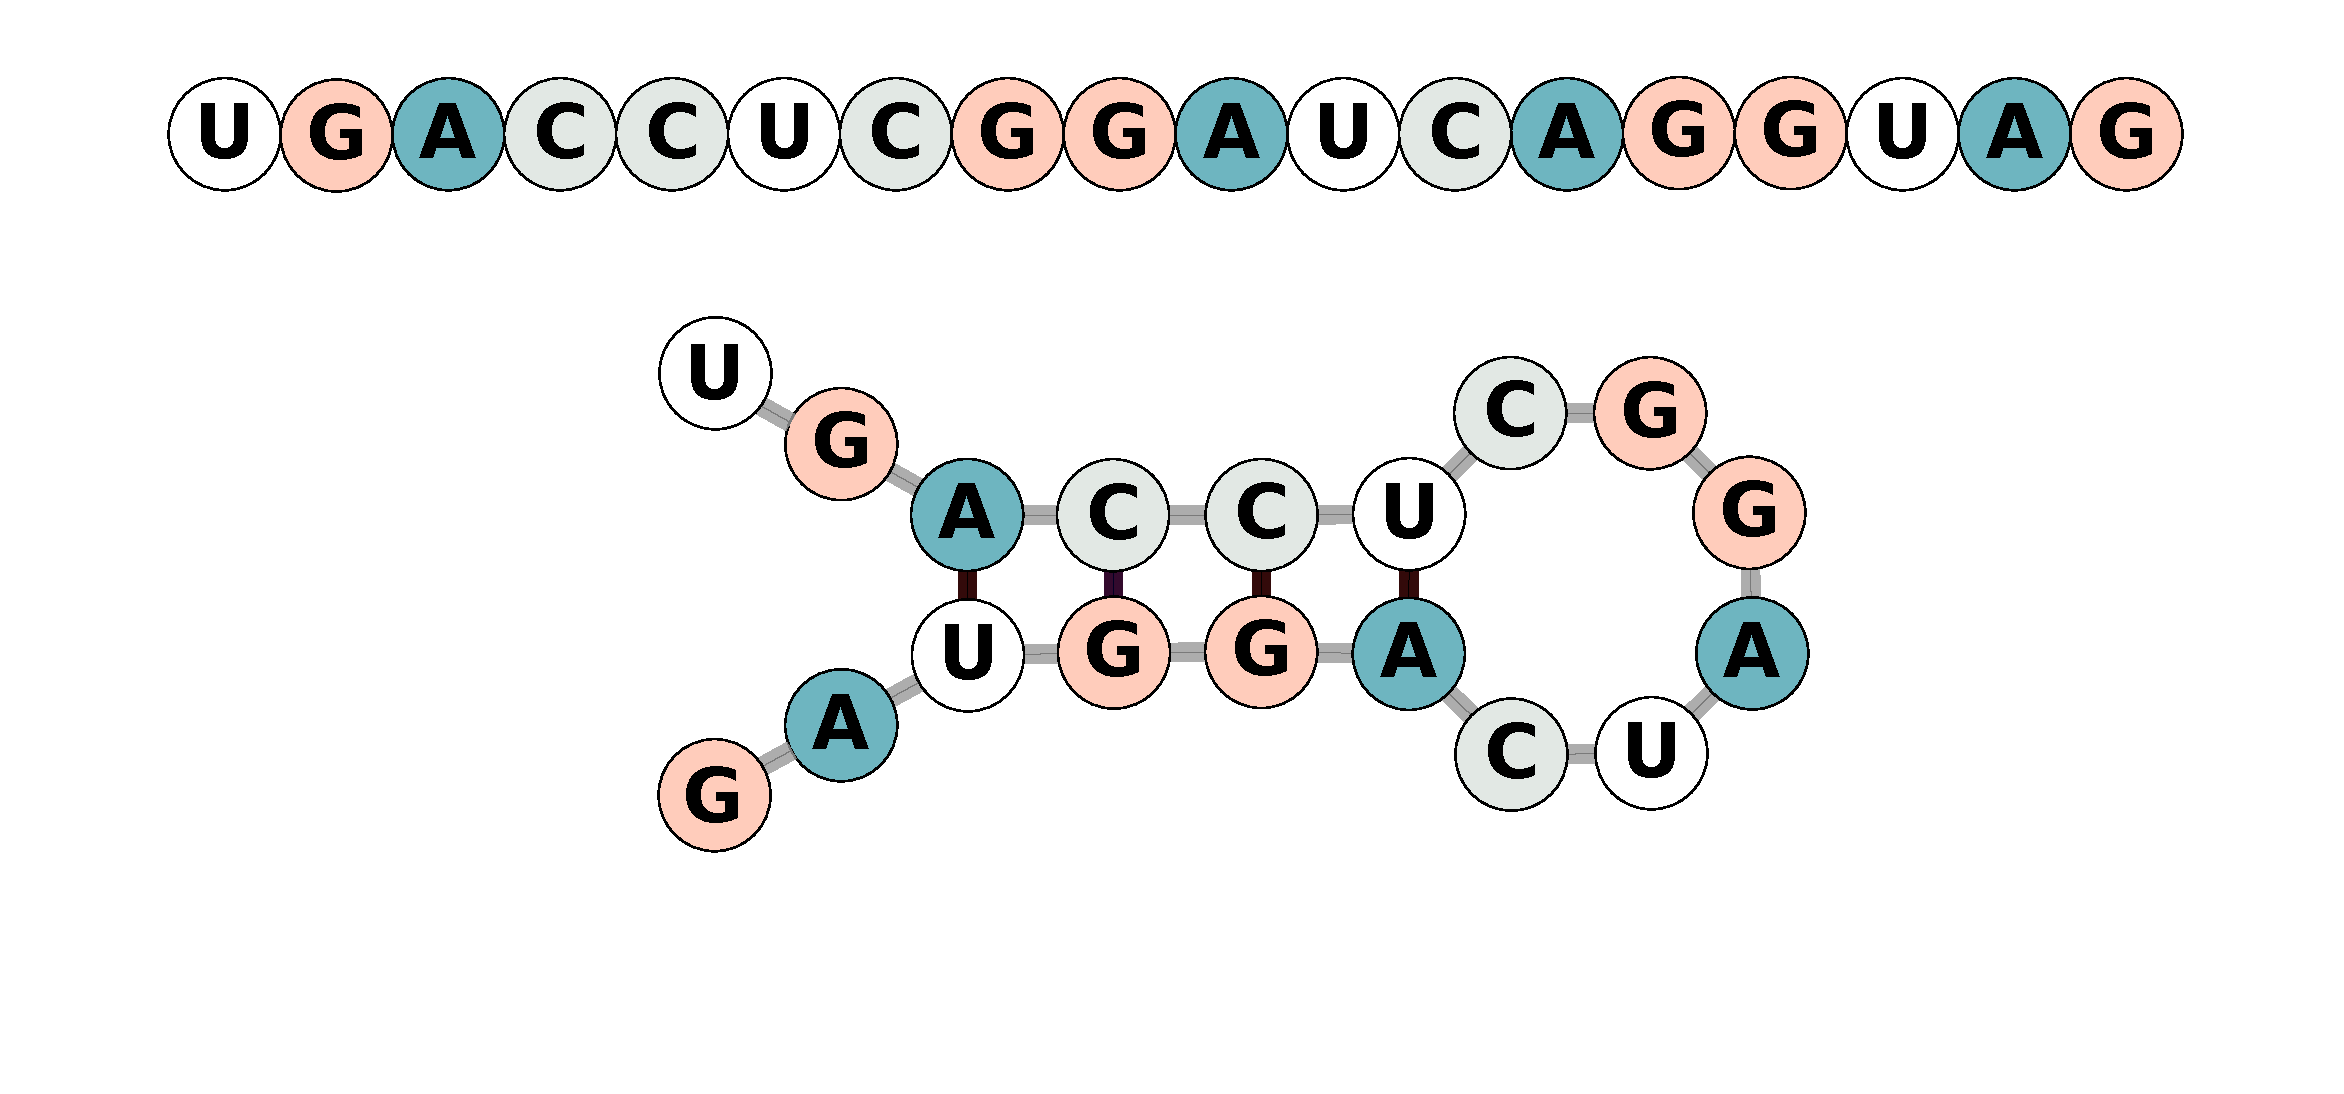
\includegraphics[width=7.7cm]{pics/stem.pdf}}
  \caption{Простая шпилька}
  \label{rna_a}
\end{subfigure}%
\begin{subfigure}{.5\textwidth}
  \centering
  \fbox{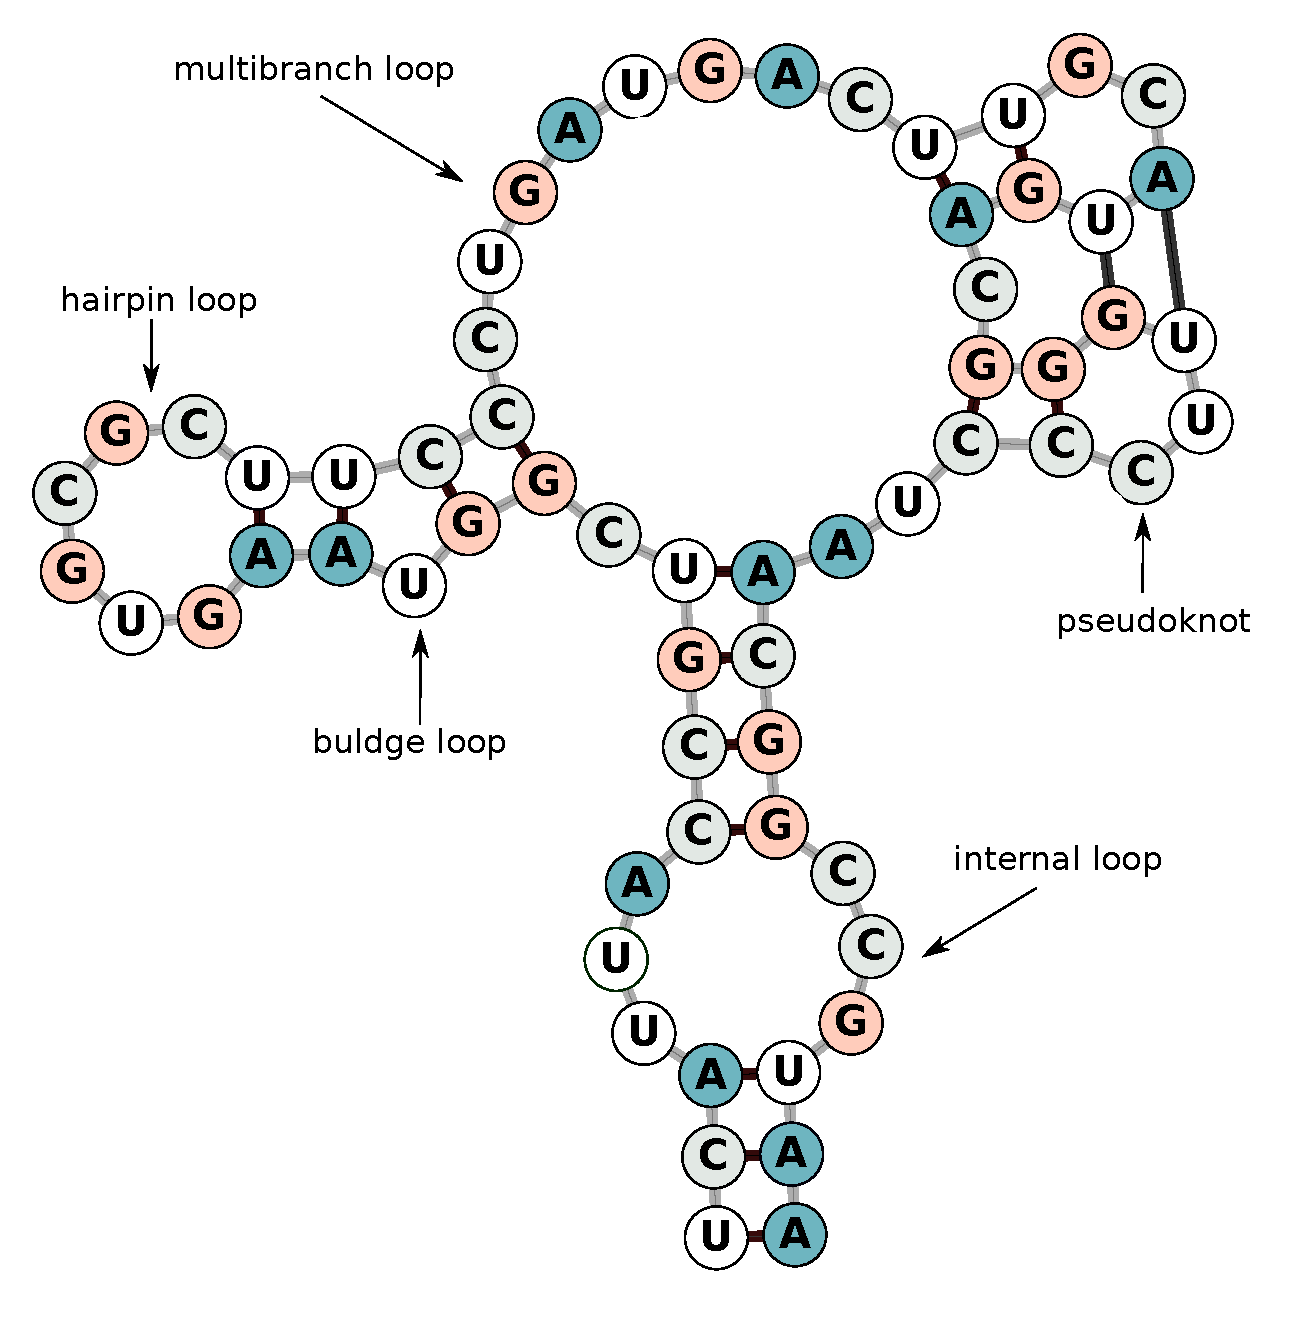
\includegraphics[width=7.7cm]{pics/rna.pdf}}
  \caption{Многообразие элементов}
  \label{rna_b}
\end{subfigure}
\caption{Вторичная структура РНК}
\label{rna}
\end{figure}

Различные исследования свойств и особенностей вторичной структуры РНК показали, что она активно участвует в таких процессах регуляции генома, как транскрипция и трансляция~\cite{wada1986local}, а также играет важную роль для филогенетического и таксономического анализа последовательностей~\cite{vrehakova2014variation,miladi2017rnascclust}, поэтому точное предсказание вторичной структуры РНК по ее нуклеотидной цепи относится к ключевым задачам современной геномики, которая усложняется тем, что вторичная структура обладает широкой вариативностью и в большинстве случаев не описывается исключительно через композицию простых шпилек, образованных Уотсон-Криковскими парами, а содержит более нетривиальные элементы.

\subsection{Подходы к предсказанию вторичной структуры РНК}
Существует большое количество  методов для предсказания вторичной структуры РНК, основанных на совершенно разных концепциях и технологиях. Самыми точными являются результаты, полученные в лабораторных условиях, например с помощью рентгеноструктурного анализа~\cite{westhof2015twenty} или ядерного магнитного резонанса~\cite{furtig2003nmr}, тем не менее, высокая цена и сложность постановки таких экспериментов приводят к активному развитию альтернативных методов --- вычислительных.

Вычислительные методы предсказания вторичных структур можно поделить на две основные группы. К первой относятся техники сравнительного анализа гомологичных последовательностей, основанные на идее о том, что биологически важные вторичные структуры не сильно меняются в процессе эволюции, поэтому сохранение двух довольно удаленных друг от друга нуклеотидов указывает на наличие водородной связи между ними во вторичной структуре~\cite{gutell2002accuracy,chen1999rna}. Такого рода результаты представляются достаточно надежными и часто используются в качестве эталонных в различных экспериментах, однако данный подход требует значительного объема ручной работы по выравниванию последовательностей и наличия достаточного количества родственных РНК для каждого вида, что далеко не всегда реализуемо на практике. Вторая и наиболее интересная в рамках данной работы группа объединяет все методы, предсказывающие вторичную структуру для единичной последовательности РНК путем построения некоторой описывающей ее физической или математической модели и решения проблемы ее оптимизации. 
Одним из самых популярных здесь подходов является принцип минимизации свободной энергии, основанный на требовании термодинамической стабильности вторичной структуры. Для решения задачи минимизации энергии могут применяться разные техники, в частности, динамическое программирование~\cite{bellaousov2013rnastructure,rivas1999dynamic}, эвристические алгоритмы~\cite{ren2005hotknots,ruan2004ilm} или иные оптимизационные схемы~\cite{reeder2007pknotsrg, jabbari2018knotty}. Кроме того, существует ряд методов, не основанных на физически измеряемых параметрах, в частности, часто максимизируется на всем пространстве вторичных структур некоторая функция оценки точности предсказания~\cite{hamada2009prediction,sato2009centroidfold} или используются стохастические контекстно-свободные грамматики для вероятностного моделирования вторичной структуры~\cite{knudsen1999rna,dowell2004evaluation}. 

Теоретическое понимание механизмов свертки последовательностей РНК и практическая реализация соответствующей модели являются достаточно нетривиальными задачами, что стало поводом к активному внедрению различных техник машинного обучения в процесс разработки алгоритмов предсказания вторичных структур как в качестве способа оценки оптимизируемых строгим алгоритмом параметров~\cite{akiyama2018max,do2006contrafold}, так и в качестве основного используемого метода~\cite{singh2019rna,apolloni2003rna}.

Несмотря на быстрое развитие идей и технологий в области вычислительной геномики, на данный момент проблема предсказания вторичной структуры молекулы РНК остается открытой, и основными сложностями при разработке алгоритмов являются предсказание псевдоузлов, неканонических пар оснований и обработка длинных последовательностей.

\subsection{Используемые технологии}
Предлагаемый в данной работе подход основан на комбинировании методов синтаксического анализа и машинного обучения, и в данном разделе будут введены основные используемые далее понятия из этих двух областей.

\subsubsection{Синтаксический анализ}
Алфавитом называется любое конечное непустое множество символов, и если $V$ --- алфавит, то через $V^\ast$ обозначается множество всех строк, составленных из символов $V$, а $L \subseteq V^\ast$  называется языком над алфавитом $V$. Для описания структуры конкретного языка, т.е. для выделения определенного подмножества из множества всех строк заданного алфавита, используется абстракция, именуемая грамматикой.

В задании правил грамматики участвуют терминальные символы, т.е. элементарные единицы некоторого языка, и нетерминальные --- синтаксические переменные, которые могут быть заменены группами терминальных символов. Формально, грамматикой называется четверка $G = (V_T, V_N, P, S)$, где $V_T$ ---  алфавит терминалов, $V_N$ --- алфавит нетерминалов, через $P$ обозначается конечное множество правил вида $\alpha \rightarrow \beta$, где $\alpha \in V^\ast V_N V^\ast$, $\beta \in V^\ast$, $V = V_N \cup V_T$, а $S$ --- стартовый нетерминал грамматики, т.е. тот нетерминал, из которого могут быть получены все предложения задаваемого ей языка. В теории формальных языков описаны различные классы грамматик, и в данной работе интерес для нас будут представлять контекстно-свободные грамматики, в которых для каждого правила $\alpha \rightarrow \beta$ выполняется условие $\alpha \in V_N$.

Строка $w$ называется выводимой из нетерминального символа $N$ грамматики $G$, если $w$ может быть получена из $N$ путем применения некоторой последовательности правил из множества правил $P$. Для автоматизации проверки выводимости строк используются различные алгоритмы синтаксического анализа, среди которых важное место занимают табличные алгоритмы, в процессе работы заполняющие для строки $w$ и нетерминала грамматики $N$ особую матрицу --- матрицу разбора $M_N$, в которой $M_N[i][j] = 1$ тогда и только тогда, когда подстрока $w[i..j]$ выводима из $N$. Самым известным табличным алгоритмом, работающим с контекстно-свободными грамматиками, является CYK~\cite{cocke1969programming,younger1967recognition,kasami1966efficient}, на ключевых принципах работы которого основываются и многие современные алгоритмы.

В рамках исследовательского проекта YaccConstructor~\cite{yacc} лаборатории языковых
инструментов JetBrains~\cite{jetbrains} проводятся исследования в области формальных языков. Среди прочего, в рамках данного проекта разрабатываются различные алгоритмы синтаксического анализа, и в данной работе использован алгоритм, основанный на матричных операциях~\cite{azimov2018context}, который демонстрирует высокую производительность на практике в связи с использованием параллельных вычислений.

\subsubsection{Машинное обучение}
К машинному обучению относятся методы создания компьютерных систем, способных находить закономерности в больших объемах данных через некоторым образом организованный процесс самостоятельного обучения. Один из таких методов --- нейронные сети --- повсеместно применяется в науке и технике, и концептуальной основой для построения обучаемой математической модели в данном случае являются принципы работы нейронов человеческого мозга.

При проектировании нейросети в первую очередь следует определить ее архитектуру, и одной из классических архитектур являются сверточные нейронные сети (convolutional neural networks), обрабатывающие, как правило, различного рода изображения. Такие сети работают на основе фильтров, которые отвечают за распознавание определенных характеристик изображения. Фильтр --- это коллекция ядер свертки, т.е. небольших матриц из чисел (весов), которые заранее неизвестны и устанавливаются в процессе обучения. Такие матрицы обрабатывают изображения по фрагментам с целью обнаружения искомых характеристик, осуществляя операцию свертки, которая является суммой произведений элементов фильтра и матрицы входных сигналов. Для решения сложных задач с многоуровневым выявлением признаков на практике требуются многослойные сверточные сети, которые часто оказывается затруднительно оптимизировать --- с увеличением глубины начинает падать точность вследствие особенностей алгоритмов обновления весов. Для решения этой проблемы была предложена особая архитектура --- остаточные нейронные сети (residual neural networks)~\cite{he2016deep}, --- основанная на добавлении дополнительных соединений быстрого доступа между блоками слоев, что упрощает процесс обучения на начальных этапах и позволяет улучшать точность результата с увеличением глубины. 

Помимо архитектуры, важным аспектом разработки нейронной сети является определение минимизируемой в процессе обучения функции ошибки (loss function), а также подбор оптимальных гиперпараметров, к которым относятся число слоев и нейронов в них, коэффициент скорости обучения (learning rate), число итераций обучения, функция активации, размер батча, способ разделения данных на обучающую и тестовую выборки и т.д. Качество работы нейросети оценивается по результатам вычисления различных метрик на тестовой выборке.

Существует множество платформ для создания и обучения нейронных сетей, и в данной работе были использованы написанные на языке Python библиотека Keras~\cite{chollet2015keras} и фреймворк Tensorflow~\cite{tensorflow2015-whitepaper}, так как данные технологии сочетают в себе удобство использования и высокую производительность.
